\documentclass[12pt]{ctexart}

% 包含必要的包
\usepackage[utf8]{inputenc}
\usepackage{amsmath, amssymb}  % 数学符号包
\usepackage{graphicx}  % 插入图片的包
\usepackage{hyperref}  % 生成超链接
\usepackage{fancyhdr}  % 页眉页脚设置
\usepackage{geometry}  % 页面设置
\usepackage{titlesec}  % 用于自定义 section 的格式
\usepackage{float}
\usepackage{listings}
\usepackage{xcolor}

\geometry{a4paper, margin=1in}

\titleformat{\section}[hang]{\normalfont\Large\bfseries}{\thesection}{1em}{}

\lstset{
    language=Python,
    basicstyle=\ttfamily\small,
    keywordstyle=\color{blue},
    stringstyle=\color{red},
    commentstyle=\color{green!50!black},
    numbers=left,
    numberstyle=\tiny\color{gray},
    frame=single,
    breaklines=true,
    backgroundcolor=\color{gray!10},
    showstringspaces=false,
    % captionpos=b % 让代码标题出现在代码下方
}

% Header and footer
\setlength{\headheight}{14.49998pt}
\addtolength{\topmargin}{-2.49998pt}

\pagestyle{fancy}
\fancyhf{}
\fancyhead[L]{《大数据分析》作业报告}
% \fancyhead[M]{清华大学}
\fancyhead[R]{刘昱杉 2024214103}
\fancyfoot[C]{\thepage}



\begin{document}

\begin{titlepage}
    \begin{center}
        % Insert logo
        
\includegraphics[width=5cm]{tsinghua_logo.png}\\[4cm]  % 插入图标并设置下方间距
        {\Huge 作业二:矩阵分解} \\[4cm]
        {\large 刘昱杉  \ \  2024214103}\\[6cm]
        {\normalsize \today}\\[1cm]
        % \vfill
        % \text{关于本实验报告对应的源码及实验环境,详见\texttt{readme}}

    \end{center}
\end{titlepage}

\section*{一、数据准备}

本次作业中,我们使用Netflix数据集,数据集被分成训练集\texttt{netflix\_train.txt}和测试集\texttt{netflix\_test.txt}。每一行的格式为\texttt{user\_id, movie\_id, rating},表示用户\texttt{user\_id}对电影\texttt{movie\_id}的评分为\texttt{rating}。
数据准备主要包括:
\begin{itemize}
    \item \textbf{数据加载}:使用\texttt{pandas}库加载数据集。
    \item \textbf{索引映射}: 为用户ID和电影ID创建唯一映射,并将ID映射为索引,便于后续矩阵运算。
    \item \textbf{稀疏矩阵创建}: 将评分数据转换为稀疏矩阵\texttt{coo\_matrix},其中行为用户,列为电影,值为评分。
\end{itemize}

这里使用了\textbf{完整的数据集},即训练集和测试集的数据都被加载,以便后续的矩阵分解模型训练和评估。

\section*{二、协同过滤与评价指标}

本作业中的协同过滤算法通过计算\textbf{用户相似度矩阵}实现,通过余弦相似度计算。
具体来说,首先对用户评分矩阵归一化,之后计算用户之间的点积。评分预测通过对\textbf{最相似的k个用户}的评分进行平均来实现。

评价指标选用均方根误差(RMSE)结果,本作业中通过对测试集上计算协同过滤方法的RMSE,最终得到值为\textbf{1.1021}。
整个流程包括:计算用户相似度、预测评分、评估RMSE,对整个测试集的计算耗时约\textbf{0.85s}。计算过程通过 PyTorch 进行了优化,以确保计算效率。

关于公式到矩阵计算的推导如下:

假设有用户-电影评分矩阵 $R \in \mathbb{R}^{m \times n}$,其中 $m$ 为用户数量,$n$ 为物品数量。用户 $i$ 对物品 $j$ 的评分为 $r_{ij}$。协同过滤通过计算用户之间的相似度矩阵 $S \in \mathbb{R}^{m \times m}$,使用如下的余弦相似度公式:

\begin{equation}
    s_{ij} = \frac{R_i \cdot R_j}{\|R_i\| \cdot \|R_j\|},
\end{equation}

其中,$R_i$ 和 $R_j$ 分别表示用户 $i$ 和用户 $j$ 的评分向量。归一化后,用户评分矩阵可以表示为:

\begin{equation}
    \hat{R}_i = \frac{R_i}{\|R_i\|},
\end{equation}

相似度矩阵 $S$ 则可以通过矩阵乘法表示为:

\begin{equation}
    S = \hat{R} \hat{R}^T,
\end{equation}

其中 $\hat{R}$ 为归一化后的用户评分矩阵。通过这个相似度矩阵,我们可以计算用户 $u$ 对电影 $j$ 的预测评分 $\hat{r}_{uj}$,方法是对最相似的 $k$ 个用户的评分取加权平均:

\begin{equation}
    \hat{r}_{uj} = \frac{\sum_{i \in N_k(u)} s_{ui} r_{ij}}{\sum_{i \in N_k(u)} s_{ui}},
\end{equation}

其中 $N_k(u)$ 表示与用户 $u$ 最相似的 $k$ 个用户集合,$s_{ui}$ 为用户 $u$ 和用户 $i$ 之间的相似度。

\section*{三、矩阵分解}

矩阵分解模型同样基于\texttt{Pytorch}实现,主要包括\textbf{User-Item Embedding}和\textbf{USer- Item Bias},可以更好地捕捉特定特征;同时防止过拟合添加了Dropout项。
训练模型使用\textbf{AdamW}优化器,学习率设置为0.01,空间维度设置为50,正则化参数$\lambda$设置为0.01,训练轮数为50。
训练过程中分别记录每5次epoch的loss和测试集上的RMSE,基于此参数下的RMSE为\textbf{0.9187}。分别在训练集和测试集上进行RMSE计算并进行曲线绘制如下。

\begin{figure}[H]
    \centering
    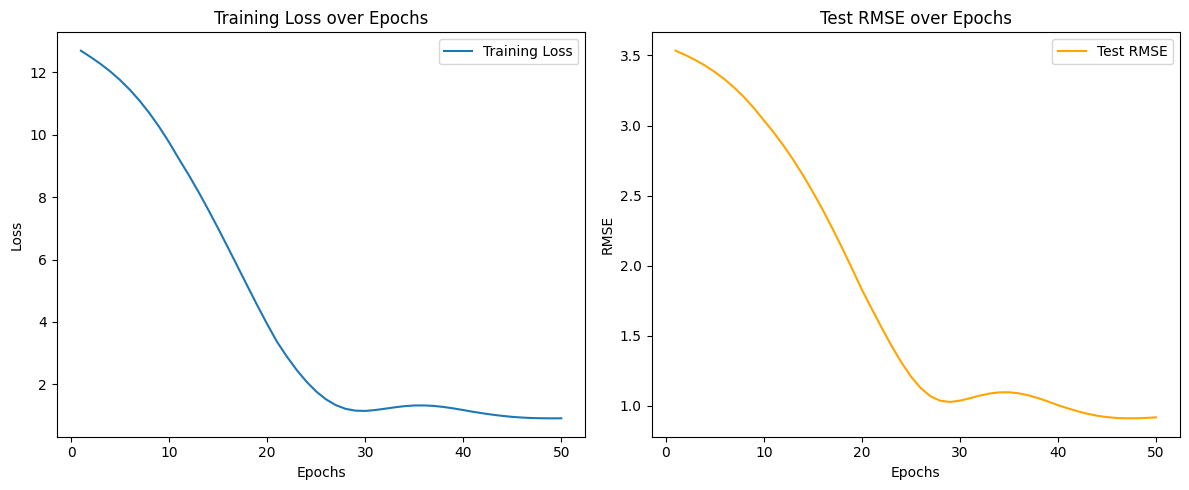
\includegraphics[width=0.8\textwidth]{image/output1.png}
    \caption{训练集和测试集上的RMSE曲线}
\end{figure}

\subsection*{参数调优}

分别使用不同的空间维度和正则化参数进行调优,并分别比较其在测试集上的RMSE值,结果如下。
由原理可知,更高的 $k$ 值可以捕捉更多特征,前期下降的更快,但到一定程度后效果会趋于平稳。增加 $\lambda$ 有助于防止过拟合,但过高的值会阻碍模型学习。
其中最佳参数组合为:空间维度$k=50$,正则化参数$\lambda=0.001$,测试集RMSE为0.9241。

\begin{table}[H]
    \centering
    \begin{tabular}{|c|c|c|}
        \hline
        空间维度$k$ & 正则化参数$\lambda$ & 测试集RMSE \\
        \hline
        20 & 0.001 & 0.9804 \\
        20 & 0.01 & 0.9806 \\
        20 & 0.1 & 0.9857 \\
        50 & 0.001 & 0.9241 \\
        50 & 0.01 & 0.9314 \\
        50 & 0.1 & 0.9319 \\
        \hline
    \end{tabular}
    \caption{不同参数下的测试集RMSE}
\end{table}

\section*{四、比较与讨论}

通过对协同过滤和矩阵分解模型的比较,可以发现矩阵分解模型在测试集上的RMSE值更低,更好地捕捉潜在的交互关系。
同时,由于协同过滤模型的计算复杂度较高,因此在计算效率上矩阵分解模型更具优势。

协同过滤和矩阵分解各有优劣,其各自的优缺点分别如下:

\subsubsection*{协同过滤}

\begin{itemize}
    \item 优点:简单易实现,不需要额外的特征工程,可以捕捉用户之间的相似度。
    \item 缺点:协同过滤对于稀疏数据不够鲁棒,且当用户数量庞大时,计算相似度矩阵的开销很大,影响效率。
\end{itemize}

\subsubsection*{矩阵分解}

\begin{itemize}
    \item 优点:矩阵分解模型可以更好地捕捉用户和物品之间的交互关系,同时可以通过添加特征更好地解释模型。通过降低矩阵维度,矩阵分解适用于大型数据集,具有良好的扩展性。
    \item 缺点:矩阵分解模型需要额外的特征工程,且其性能对超参数(如嵌入维度、正则化系数等)较为敏感。
\end{itemize}



\newpage

\begin{thebibliography}{9}
    \bibitem{collaborative_filtering} 
    Su, X., \& Khoshgoftaar, T. M. (2009). A survey of collaborative filtering techniques. \textit{Advances in Artificial Intelligence}, 2009.
    
    \bibitem{matrix_factorization} 
    Koren, Y., Bell, R., \& Volinsky, C. (2009). Matrix factorization techniques for recommender systems. \textit{Computer}, 42(8), 30-37.
    
    \bibitem{pytorch} 
    Paszke, A., Gross, S., Massa, F., Lerer, A., Bradbury, J., Chanan, G., ... \& Chintala, S. (2019). PyTorch: An imperative style, high-performance deep learning library. \textit{Advances in Neural Information Processing Systems}, 32.
    
    \bibitem{myself} 
    ChatGPT, OpenAI. (2024). Implementation and comparison of collaborative filtering and matrix factorization in recommendation systems.
\end{thebibliography}

\end{document}
